\documentclass[10pt]{article}
\usepackage[a4paper,margin=0.72in,top=0.6in,bottom=0.65in]{geometry}
\usepackage[T1]{fontenc}
\usepackage{lmodern}
\usepackage{microtype}
\usepackage{graphicx}
\usepackage{booktabs}
\usepackage{tabularx}
\usepackage{amsmath,amssymb}
\usepackage{xurl}
\usepackage[dvipsnames]{xcolor}
\usepackage{tikz}
\usetikzlibrary{arrows.meta,positioning,fit}
\usepackage{enumitem}
\usepackage{titlesec}
\usepackage[hidelinks]{hyperref}
\usepackage{tcolorbox}
\usepackage{caption}
\usepackage{fancyhdr}

\definecolor{ink}{HTML}{1A2B4C}
\definecolor{accent}{HTML}{2B6CB0}
\definecolor{hot}{HTML}{C53030}
\definecolor{soft}{HTML}{EEF3FA}

\titleformat{\section}{\large\bfseries\color{ink}}{\thesection}{0.6em}{}
\titlespacing*{\section}{0pt}{7pt}{3pt}
\titleformat{\subsection}{\normalsize\bfseries\color{ink}}{\thesubsection}{0.5em}{}
\titlespacing*{\subsection}{0pt}{5pt}{2pt}
\setlist{nosep,leftmargin=1.2em}
\captionsetup{font=small,labelfont={bf,color=ink},skip=3pt}
\setlength{\parskip}{3pt}
\setlength{\parindent}{0pt}
\setlength{\textfloatsep}{6pt}
\setlength{\intextsep}{5pt}

\pagestyle{fancy}
\fancyhf{}
\renewcommand{\headrulewidth}{0pt}
\fancyfoot[L]{\footnotesize\color{gray}Chirayu \textbar{} GIFT FutureLab Grand Challenge 2026--27 \textbar{} First-shortlist submission}
\fancyfoot[R]{\footnotesize\color{gray}\thepage/4}

\newcommand{\num}[1]{\textbf{#1}}

\begin{document}

%================ HEADER =================
{\color{ink}\noindent
{\footnotesize\textbf{TEAM:} Team Chirayu \quad\textbf{MEMBERS:} Kalp Shah, Harsh Dhru (IIT Gandhinagar)}\\[3pt]
{\LARGE\bfseries Chirayu: condition-priced GPU leases and lease-backed financing from GIFT IFSC}\\[2pt]
{\small Code and data: \url{https://github.com/kalpshah18/Chirayu}}}
\vspace{4pt}

\begin{tcolorbox}[colback=soft,colframe=accent,boxrule=0.6pt,arc=2pt,left=6pt,right=6pt,top=4pt,bottom=4pt]
\small
\textbf{The financial problem.} IFSCA's October 2026 notification lets GIFT IFSC units lease GPUs the way they lease aircraft \cite{ifsca}. What such a lease costs to finance is set by what the GPU is worth when it comes back, and that depends on how hard it was run, which nobody measures today.
\textbf{What we built.} Chirayu meters each leased GPU's operating condition through tamper-evident telemetry and turns it into rent, wear reserves, monthly marks and tranche sizes for the lessor and its lenders.
\textbf{Result on real fleet data.} On 30,207 GPUs of the Titan supercomputer, identical cards in the hottest cabinet position failed at \num{13.8$\times$} the rate of those in the coolest (Cox model, controlling for manufacturing batch and position on the blade): \num{22.5\%} vs \num{1.3\%} were dead within a 36-month lease term. When a lessor charges one flat rent and its book fills with hard-running lessees, it loses \num{4.3\%} of its residual exposure on average and \num{7.6\%} at the 99th percentile. Pricing each lease on condition removes the expected loss and cuts the 99th-percentile loss to \num{3.3\%}.
\end{tcolorbox}

%================ SECTION 1 =================
\section{Technical contribution and progress}

\subsection{The problem in finance terms}
On 22 October 2026 IFSCA notified GPUs, AI accelerators and dedicated data-centre equipment as a financial product in IFSC (Notification IFSCA/GN/2026/017), opening operating leases of GPUs from GIFT City \cite{ifsca}. The template is aircraft leasing, where GIFT IFSC already hosts 38 registered lessors and 196 leased aircraft \cite{kpmg}. Demand is domestic and large: the IndiaAI Mission has onboarded over 38,000 GPUs \cite{indiaai}. Market hedges are on their way: CME with Silicon Data and ICE with Ornn have announced GPU rental-index futures, though neither has started trading while US regulators review them \cite{cme,ice}.

A lessor's return on a GPU lease depends on the GPU's value when it comes back. That value depends on how hard the GPU was run, and today nobody prices that. The used market already pays 15--30 points more for tested, refurbished H100s than for as-is units, and the gap widens with age \cite{silicondata}, yet no public market or dataset ties resale price to usage \cite{silicondata,wing}. Lenders therefore lean on contracted cash flows and full amortisation rather than on the hardware \cite{wing}. The same blind spot creates adverse selection: under one flat rent, lessees who run their GPUs gently subsidise those who run them hot, and the gentle ones have reason to leave.

\subsection{The part we chose to show: from measured condition to price and loss}
Chirayu has four layers (Figure~\ref{fig:arch}). We present the \emph{condition-to-price engine}, because it is the step that turns engineering data into a financial number, and because we could calibrate it on real fleet data without a GPU of our own.

\begin{figure}[h]
\centering
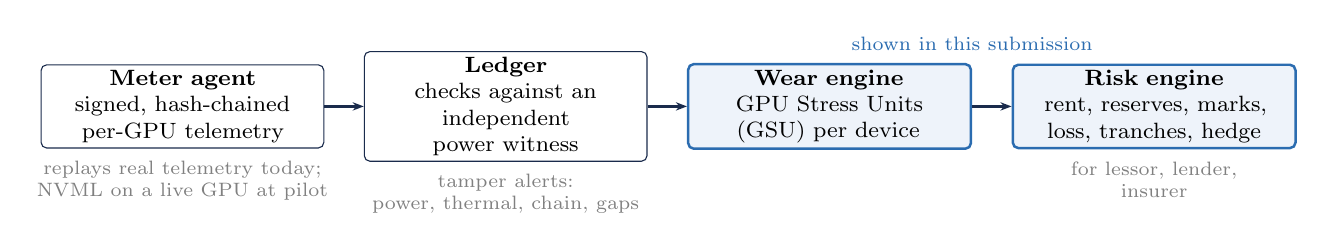
\begin{tikzpicture}[
  box/.style={draw=ink,rounded corners=2pt,fill=white,align=center,font=\footnotesize,minimum height=1.05cm,text width=3.45cm,inner sep=2pt},
  hl/.style={box,fill=soft,draw=accent,line width=0.9pt},
  arr/.style={-{Stealth[length=4pt]},ink,thick},
  lab/.style={font=\scriptsize\color{gray},align=center}]
\node[box] (a) {\textbf{Meter agent}\\signed, hash-chained\\per-GPU telemetry};
\node[box,right=0.5cm of a] (l) {\textbf{Ledger}\\checks against an\\independent power witness};
\node[hl,right=0.5cm of l] (w) {\textbf{Wear engine}\\GPU Stress Units\\(GSU) per device};
\node[hl,right=0.5cm of w] (r) {\textbf{Risk engine}\\rent, reserves, marks,\\loss, tranches, hedge};
\draw[arr] (a) -- (l); \draw[arr] (l) -- (w); \draw[arr] (w) -- (r);
\node[lab,below=1pt of a] {replays real telemetry today;\\NVML on a live GPU at pilot};
\node[lab,below=1pt of l] {tamper alerts:\\power, thermal, chain, gaps};
\node[lab,below=1pt of r] {for lessor, lender,\\insurer};
\node[font=\scriptsize\color{accent},above=1pt of w.north east,anchor=south] {shown in this submission};
\end{tikzpicture}
\caption{Chirayu's pipeline. Highlighted: the part presented here.}
\label{fig:arch}
\end{figure}

\textbf{How it works.} Each GPU carries a condition state $c$: in a live lease this is its cumulative wear in GSU, and in the Titan calibration below it is the cabinet position the operator recorded. The engine values the GPU at lease end $T$ as
\[
\mathbb{E}[V_T \mid c] \;=\; \bigl(1-p_f(c)\bigr)\,M_T\,e^{-\lambda g_T} \;+\; p_f(c)\,S ,
\]
where $p_f(c)$ is the probability the card has failed by $T$ (from a survival model), $M_T$ is the market value of a healthy card, $e^{-\lambda g_T}$ discounts for accumulated wear $g_T$, and $S$ is salvage. The break-even monthly rent $B(c)$ then solves
\[
K \;=\; \sum_{m=1}^{T} \frac{B(c)}{(1+y)^m} \;+\; \frac{\mathbb{E}[V_T\mid c]}{(1+y)^T},
\]
with $K$ the purchase cost and $y$ the lessor's monthly target yield. In a live lease, rent splits into a base rent plus a \emph{wear reserve} charged per GSU, $r=-(1+y)^{-T}\,\partial\,\mathbb{E}[V_T]/\partial g$, the way aircraft lessors bill maintenance reserves per flight hour \cite{aircraft}. The GSU itself combines time at temperature and power (Arrhenius form), thermal cycles counted by rainflow \cite{twomey}, and growth in memory errors, with every parameter in the repository tagged with its source or marked as an assumption.

\subsection{Evidence on real data: identical GPUs, different conditions, very different lives}
We fitted the engine's survival layer to the public Titan GPU-lifetime dataset \cite{titan}: 30,207 NVIDIA K20X cards, 100,889 GPU-years and 5,089 failures, each with the cabinet slot it ran in. Titan blew cooling air from the bottom of each cabinet to the top, so cage~0 ran coolest and cage~2 hottest (Figure~\ref{fig:titan}, left). The original authors found that GPU reliability on Titan depends on heat dissipation tied to this cooling design \cite{titan}.

\begin{figure}[h]
\centering
\begin{minipage}[c]{0.36\linewidth}\centering
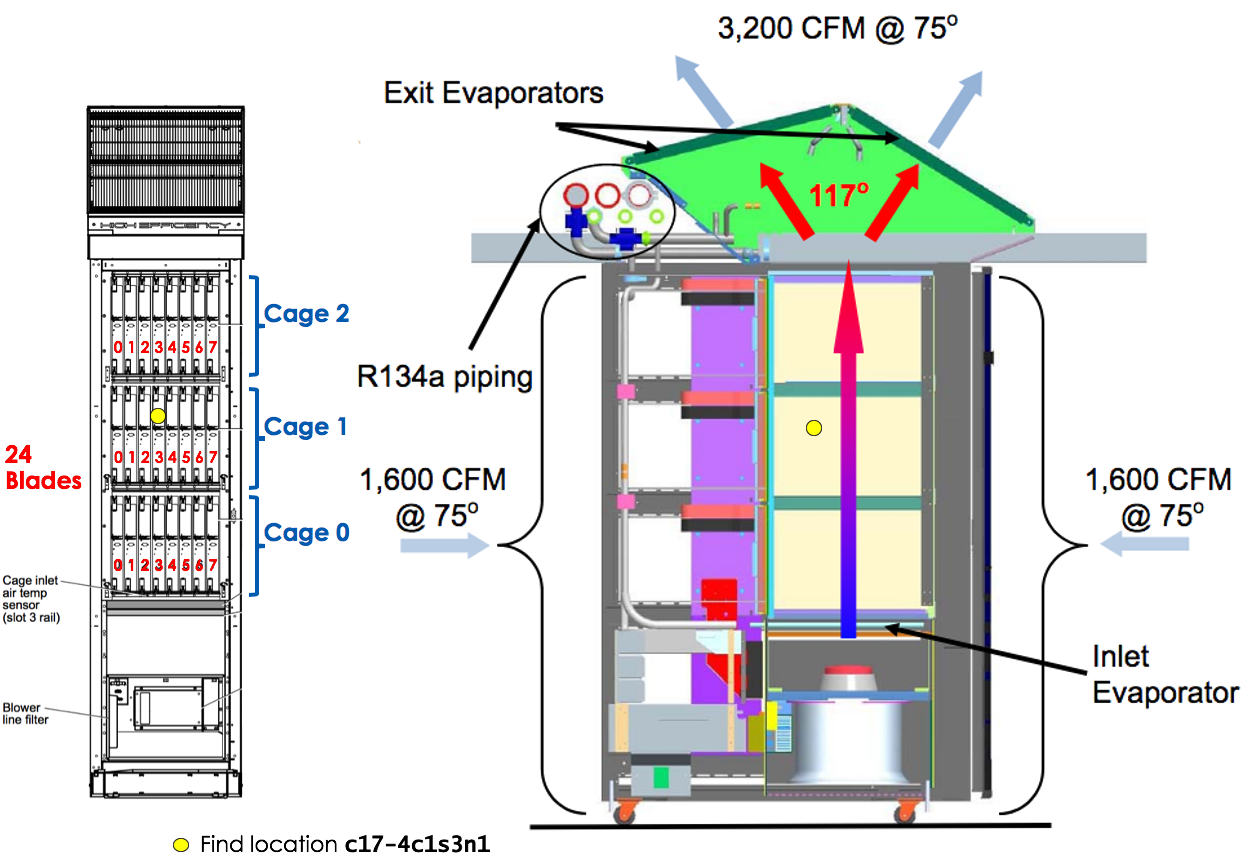
\includegraphics[width=\linewidth]{fig/TitanCabinet.png}
\end{minipage}\hfill
\begin{minipage}[c]{0.62\linewidth}\centering
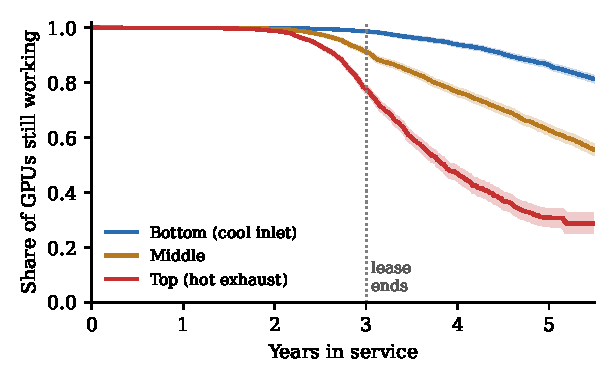
\includegraphics[width=\linewidth]{fig/km_by_cage.pdf}
\end{minipage}
\caption{Left: a Titan cabinet; air enters at the bottom and leaves the top hot (image from the dataset's repository \cite{titan}). Right: our Kaplan--Meier estimate of the share of GPUs still working, by cage, with 95\% bands.}
\label{fig:titan}
\end{figure}

\begin{table}[h]
\centering\small
\begin{tabular}{lrrrrr}
\toprule
Cage (position) & GPUs & \shortstack[r]{Failures per\\100 GPU-years} & \shortstack[r]{Failed by\\month 36} & \shortstack[r]{Cox hazard ratio\\{[95\% CI]}} & \shortstack[r]{Break-even\\monthly rent} \\
\midrule
0, bottom (cool) & 7,017 & 3.3 & 1.3\% & 1 (reference) & \$790 \\
1, middle & 10,398 & 5.3 & 8.9\% & 4.3 [4.0, 4.7] & \$803 \\
2, top (hot) & 12,792 & 6.5 & 22.5\% & 13.8 [12.6, 15.0] & \$827 \\
\midrule
One flat rent for all & 30,207 & 5.0 & 12.9\% & -- & \$810 \\
\bottomrule
\end{tabular}
\caption{Survival and pricing by condition. The Cox model also controls for the GPU's position on its blade and its manufacturing batch (concordance 0.78). Rent: 36-month lease of a \$30{,}000 GPU at a 12\% annual yield, healthy-card value 30\% of cost at lease end, salvage 5\%.}
\label{tab:titan}
\end{table}

\subsection{Result: what condition data is worth to a lessor and its lender}
A cool-running lessee pays \$20 a month too much under the flat rent, \$724 over the term; a hot-running lessee pays \$17 too little. That cross-subsidy invites adverse selection. We simulated a 500-GPU book (50,000 paths) whose residual exposure is \$4.5\,million, in three cases (Figure~\ref{fig:tail}):

\begin{figure}[h]
\centering
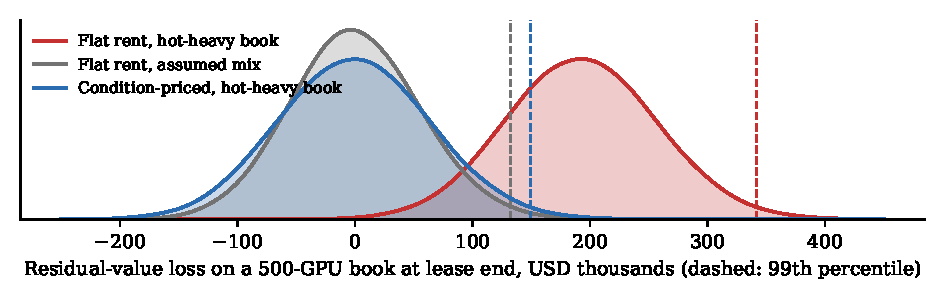
\includegraphics[width=\linewidth]{fig/tail_loss.pdf}
\vspace{-2pt}\caption{Distribution of the lessor's residual-value loss at lease end. ``Hot-heavy'' means 70\% of lessees run like cage 2, 25\% like cage 1 and 5\% like cage 0.}
\label{fig:tail}
\end{figure}

\begin{table}[h]
\centering\small
\begin{tabularx}{\linewidth}{Xrr}
\toprule
Case & Expected loss & 99th-percentile loss \\
\midrule
Flat rent, book mix as the lessor assumed & 0.0\% & 2.9\% \\
Flat rent, book fills with hot-running lessees & \textcolor{hot}{\textbf{4.3\%}} & \textcolor{hot}{\textbf{7.6\%}} \\
Condition-priced rent, same hot-heavy book & \textbf{0.0\%} & \textbf{3.3\%} \\
\bottomrule
\end{tabularx}
\caption{Loss as a share of the book's residual exposure. Condition pricing keeps the lessor whole whatever mix of lessees it attracts; the remaining tail is the true randomness of failures, which a lender can size a senior tranche against.}
\label{tab:loss}
\end{table}

\textbf{What this shows, and its limits.} Operating conditions move failure risk by an order of magnitude on identical hardware, and that difference is large enough to change rent, reserves and the size of loan a lender can safely make. Titan's cards are older (K20X) and its position effect sits on top of batch effects, which our model controls for. The calculation is also conservative: it ignores downtime and replacement of cards that fail mid-lease. For modern GPUs we anchor baseline failure rates to published H100 and A100 studies: Llama~3's training run saw 419 unexpected interruptions in 54 days on 16,384 H100s, 148 from faulty GPUs and 72 from HBM3 memory \cite{llama3}; Meta's research clusters logged 6.50 vs 2.34 failures per 1,000 node-days on two clusters \cite{kokolis}; and H100's memory MTBE was 3.2$\times$ lower than A100's on NCSA Delta \cite{cui}.

\subsection{Prototype status and what we will test next}
The full pipeline runs today in our repository: signed telemetry chain, ledger with two tamper detectors, GSU wear engine, and the risk engine (pricing, Monte Carlo with regime-switching rents and correlated lessee defaults, tranching, hedge ratio, insurance premium), with 21 passing unit tests. Three tests come next, each on a public dataset:
\begin{enumerate}
\item \textbf{Can a lessee fake its telemetry?} Summit's released telemetry (via the ClusterWise mirror, 27,756 V100s) records each GPU's self-reported power and, separately, each node's power-supply input power \cite{shin,clusterwise}. The power supplies are a separate hardware path, so they serve as our independent witness. We will inject under-reported power and temperature, deleted windows, replays and identity swaps into 200+ real nodes and measure detection rate, delay and false alarms per node-day. Our detector fits supply power against reported power with an offset and gain, because Summit's own node sums differ from switchboard meters by about 11\% on average while moving in phase \cite{shin}. \emph{We expect} to show that a 20\% power under-report is caught within an hour, and to measure how far a physically consistent fake can go before the witness catches it.
\item \textbf{How differently do real workloads wear a GPU?} MIT Supercloud's GPU traces are sampled every 100\,ms with a labelled subset of deep-learning jobs \cite{supercloud}. We will cluster jobs into lessee archetypes and compute each archetype's GSU distribution; \emph{we expect} steady training and bursty experimentation to rank differently on wear and therefore on rent.
\item \textbf{What can a lessee do about it?} Power capping on the same cluster lowered GPU temperature by about 4.8\,$^\circ$C on average \cite{zhao}. We will turn this into a lessee-side tool: the power cap that minimises energy cost plus wear reserve minus lost throughput.
\end{enumerate}

%================ SECTION 2 =================
\section{Papers and references}
\vspace{-2pt}
\begingroup
\renewcommand{\section}[2]{}
\small
\begin{thebibliography}{99}\setlength{\itemsep}{1pt}

\bibitem{ifsca} IFSCA. \emph{Notification on GPU and connected data centre equipment as a financial product in IFSC}, IFSCA/GN/2026/017, 22 Oct 2026. \url{https://www.ifsca.gov.in/home/NewSection}
\bibitem{kpmg} KPMG India. \emph{Advancing the aircraft leasing ecosystem in India}, May 2026. \url{https://assets.kpmg.com/content/dam/kpmgsites/in/pdf/2026/05/advancing-the-aircraft-leasing-ecosystem-in-india-from-reforms-to-powering-future-growth.pdf}
\bibitem{indiaai} IndiaAI Mission onboards 38,000+ GPUs (Lok Sabha reply, 25 Mar 2026), via \url{https://www.devdiscourse.com/article/law-order/3850323-10372-cr-indiaai-mission-onboards-38000-gpus-190-projects-approved}
\bibitem{cme} CME Group. Compute futures on Silicon Data H100/B200 rental indices (press releases, 12 May and 11 Aug 2026). \url{https://cmegroup.com/markets/energy/power/compute-futures.html}
\bibitem{ice} ICE. \emph{ICE and Ornn to launch GPU compute futures contracts}, 19 May 2026. \url{https://ir.theice.com/press/news-details/2026/ICE-and-Ornn-to-Launch-GPU-Compute-Futures-Contracts/default.aspx}
\bibitem{titan} G.~Ostrouchov, D.~Maxwell, R.~A.~Ashraf, C.~Engelmann, M.~Shankar, J.~H.~Rogers. GPU lifetimes on Titan supercomputer: survival analysis and reliability. \emph{SC20}. Data and code: \url{https://github.com/olcf/TitanGPULife}; \url{https://www.osti.gov/biblio/1657202}
\bibitem{shin} W.~Shin, V.~Oles, A.~M.~Karimi, J.~A.~Ellis, F.~Wang. Revealing power, energy and thermal dynamics of a 200PF pre-exascale supercomputer. \emph{SC21}. DOI 10.1145/3458817.3476188. Dataset: \url{https://www.osti.gov/biblio/1861393}
\bibitem{clusterwise} ClusterWise: Summit-derived telemetry with failure labels, CC BY 4.0. DOI 10.57967/hf/9384. \url{https://huggingface.co/datasets/MachaParfait/ClusterWise}
\bibitem{supercloud} S.~Samsi et al. The MIT Supercloud dataset. arXiv:2108.02037. \url{https://dcc.mit.edu/data}
\bibitem{cui} S.~Cui et al. Story of two GPUs: characterizing the resilience of Hopper H100 and Ampere A100 GPUs. \emph{SC25}. DOI 10.1145/3712285.3759821; arXiv:2503.11901.
\bibitem{kokolis} A.~Kokolis et al. Revisiting reliability in large-scale machine learning research clusters. arXiv:2410.21680.
\bibitem{llama3} Llama Team, Meta. The Llama 3 herd of models. arXiv:2407.21783.
\bibitem{zhao} D.~Zhao et al. Sustainable supercomputing for AI: GPU power capping at HPC scale. arXiv:2402.18593.
\bibitem{twomey} K.~Twomey et al. Development of a cycle counting algorithm with temporal parameters. \emph{Microelectronics Reliability} 109 (2020). DOI 10.1016/j.microrel.2020.113652
\bibitem{silicondata} Silicon Data. \emph{H100 GPU market value trends}, Jan 2026. \url{https://www.silicondata.com/use-cases/h100-gpu-market-value-trends}
\bibitem{wing} Wing VC. \emph{How the GPU became collateral}, Sep 2026. \url{https://www.wing.vc/content/how-the-gpu-became-collateral}
\bibitem{aircraft} Acumen Aviation. \emph{Aircraft maintenance reserves explained}. \url{https://www.acumen.aero/blogs/aircraft-maintenance-reserves-explained-how-they-work-and-why-they-matter}

\end{thebibliography}
\endgroup

\textbf{Related work by team members.} A.~Kuloor, H.~Dhru, R.~Modi, K.~Shah, \emph{Fairness, efficiency, and strategic behaviour in shared GPU allocation} (manuscript, being prepared for submission; not yet published). It studies how users game the sharing of scarce GPUs, the same incentive problem that makes tamper-evident metering necessary in a lease. Our code, data-processing scripts and every number in this document are in \url{https://github.com/kalpshah18/Chirayu} (\texttt{analysis/titan\_condition\_pricing.py} reproduces Section 1.3--1.4 in under a minute).

%================ SECTION 3 =================
\section{Plan for the finale}
\textbf{What we will present.} A working risk desk for a GIFT IFSC GPU lessor, run live on one laptop, over a 500-lease book whose lessees behave like real workloads (MIT Supercloud archetypes) and whose failure risk is calibrated on real fleets (Titan, Summit) and anchored to published H100 failure rates. Every number on screen will trace to a dataset or paper and a fixed random seed.

\begin{table}[h]
\centering\small
\begin{tabularx}{\linewidth}{@{}p{3.1cm}X X@{}}
\toprule
Demo moment & What the panel sees & Financial question it answers \\
\midrule
1. The book & Marks, loan-to-value, expected and tail loss for every lease, updating as telemetry arrives & What is this lease book worth today, and how much can a bank lend against it? \\
2. Price a lease live & Same GPU-hours under two real workload profiles give two rents, next to the flat worst-case rent & What should a lessor charge, and how much does pricing on condition save a careful lessee? \\
3. What the data is worth & Senior tranche size and funding cost in basis points, with and without condition data; residual-value insurance premium both ways & How much cheaper does funding become when the collateral is measured? \\
4. Why you can trust it & A real Summit node replayed with its independent power-supply reading overlaid; we inject a 20\% power under-report live and the alert fires; then the same test across 200+ nodes (detection rate, false alarms per node-day) & Can a lessee cheat the meter that sets its rent? \\
\bottomrule
\end{tabularx}
\end{table}

\textbf{How it shows the application in finance.} The users are the institutions IFSCA's notification creates: a GIFT IFSC lessor pricing and reserving leases, an IFSC Banking Unit lending against the lease book, and an insurer writing residual-value cover. Chirayu gives each of them a number they do not have today: rent and reserves that follow measured use, monthly marks of each GPU, and a loss distribution a credit committee can size a senior tranche against. Aircraft lessors already work this way, with reserves billed per flight hour against reported usage \cite{aircraft}; Chirayu makes the equivalent usage record for GPUs, and makes it hard to falsify.

\textbf{Commitments for the finale (22 Dec 2026).} (i) Tamper-detection results on at least 200 real Summit nodes, reported with detection rate, delay and false-alarm rate, whatever they turn out to be. (ii) Lessee archetypes built from MIT Supercloud traces, with a GSU distribution for each. (iii) The value-of-data result in basis points of funding cost. (iv) Every parameter listed with its source or marked as an assumption. After the finale we want to pilot with one GIFT lessor and one Indian GPU cloud on 8--64 GPUs, where the meter runs on live hardware with a physical power witness.

\end{document}
